%%%%%%%%%%%%%%%%%%%%%%%%%%%%%%%%%%%%%%%%%%%%%%%%%%%%%%%%%%%%%%%%%%
%
% Analysis of Algorithms
%
% Homework Assignment #6
%
%%%%%%%%%%%%%%%%%%%%%%%%%%%%%%%%%%%%%%%%%%%%%%%%%%%%%%%%%%%%%%%%%%
%%%%%%%%%%%%%%%%%%%%%%%%%%%%%%%%%%%%%%%%%%%%%%%%%%%%%%%%%%%%%%%%%%
%
% Score Card and Answer Sheets
%
%%%%%%%%%%%%%%%%%%%%%%%%%%%%%%%%%%%%%%%%%%%%%%%%%%%%%%%%%%%%%%%%%%
\documentclass[addpoints,11pt]{exam}
\usepackage{clrscode4e}
\usepackage{tcucosc}
\usepackage{units}
\usepackage{enumitem}
\usepackage{hyperref}
\usepackage{fullpage}
\usepackage{tkz-berge}
\usepackage{graphicx}
\usepackage{listings}
\usepackage{amsmath}


%%%%%%%%%%%%%%%%%%%%%%%%%%%%%%%%%%%%%%%%%%%%%%%%%%%%%%%%%%%%%%%%%%
%
% Begin Document
%
%%%%%%%%%%%%%%%%%%%%%%%%%%%%%%%%%%%%%%%%%%%%%%%%%%%%%%%%%%%%%%%%%%
\begin{document}
	\pagestyle{empty}
	
	
	\noindent{\large\bfseries Name: Zachary Macadam}\\
	\noindent{\large\bfseries COSC 40403 - Analysis of Algorithms: Homework 6}\\
	\noindent{\large\bfseries Due: 23:59:59 on November 13}
	
	%%%%%%%%%%%%%%%%%%%%%%%%%%%%%%%%%%%%%%%%%%%%%%%%%%%%%%%%%%%%%%%%%%
	%
	% Score Card and Answer Sheets
	%
	% Comment out one-or-the-other to show or not-show the answers.
	%
	%%%%%%%%%%%%%%%%%%%%%%%%%%%%%%%%%%%%%%%%%%%%%%%%%%%%%%%%%%%%%%%%%%
	\printanswers
	%%\noprintanswers
	
	
	%%%%%%%%%%%%%%%%%%%%%%%%%%%%%%%%%%%%%%%%%%%%%%%%%%%%%%%%%%%%%%%%%%
	%
	% Score Card
	%
	%%%%%%%%%%%%%%%%%%%%%%%%%%%%%%%%%%%%%%%%%%%%%%%%%%%%%%%%%%%%%%%%%%
	\ifprintanswers
	\noindent
	\begin{center}
		\gradetable[v][questions]
	\end{center}
	\newpage
	\fi
	
	
	%%%%%%%%%%%%%%%%%%%%%%%%%%%%%%%%%%%%%%%%%%%%%%%%%%%%%%%%%%%%%%%%%%
	%
	% Question 1
	%
	%%%%%%%%%%%%%%%%%%%%%%%%%%%%%%%%%%%%%%%%%%%%%%%%%%%%%%%%%%%%%%%%%%
	\begin{questions}
		\question[10]
		Use Prim's algorithm to find a minimum spanning tree for the following graph.  Show the actions step by step.
		
		\includegraphics[scale=0.5]{g1.pdf}
		\begin{solutionorbox} \\ 
			Using Prim's algorithm beginning at node V1: \\
			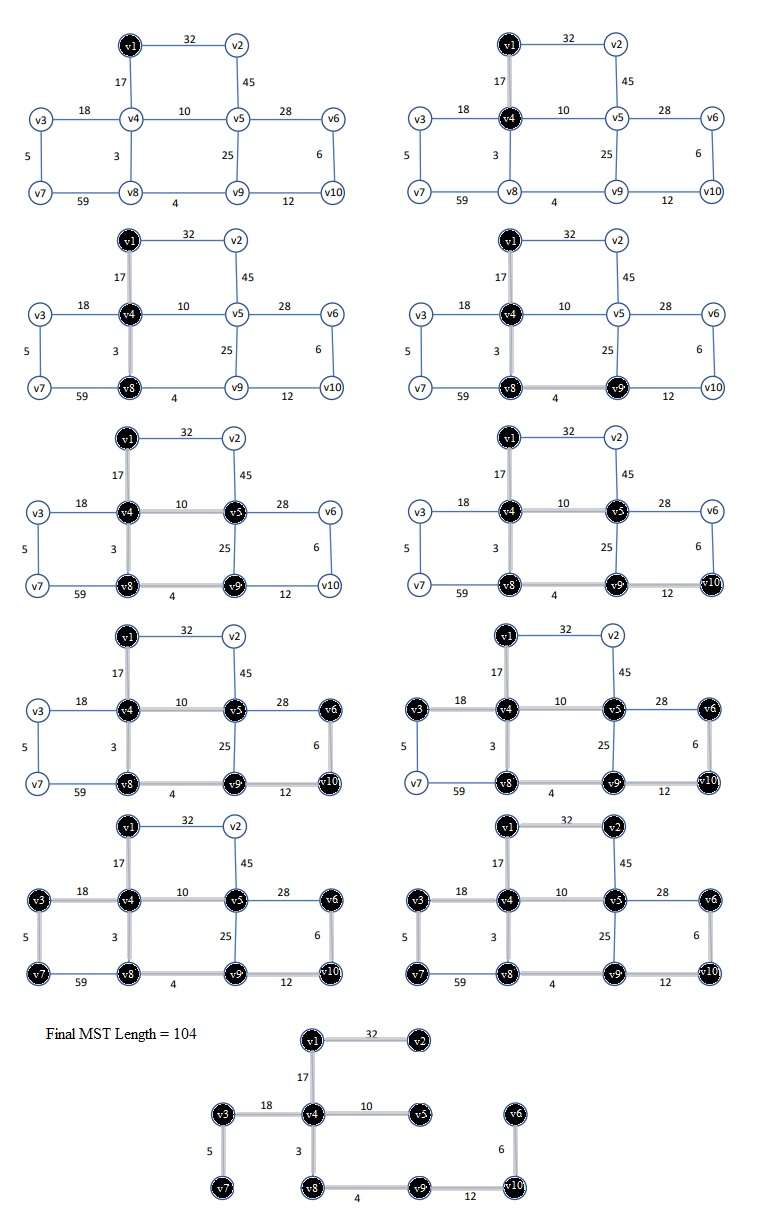
\includegraphics[width=0.7\textwidth]{prims.jpg}
		\end{solutionorbox}
		
		\ifprintanswers
		\newpage
		\else
		\bigskip
		\fi
		
		
		%%%%%%%%%%%%%%%%%%%%%%%%%%%%%%%%%%%%%%%%%%%%%%%%%%%%%%%%%%%%%%%%%%
		%
		% Question 2
		%
		%%%%%%%%%%%%%%%%%%%%%%%%%%%%%%%%%%%%%%%%%%%%%%%%%%%%%%%%%%%%%%%%%%
		\question[10]
		Use Kruskal's algorithm to find a minimum spanning tree for the graph shown above.  Show the actions step by step.
		\begin{solutionorbox} \\ 
			Using Kruskal's algorithm beginning at the minimum weight edge of weight 3: \\
			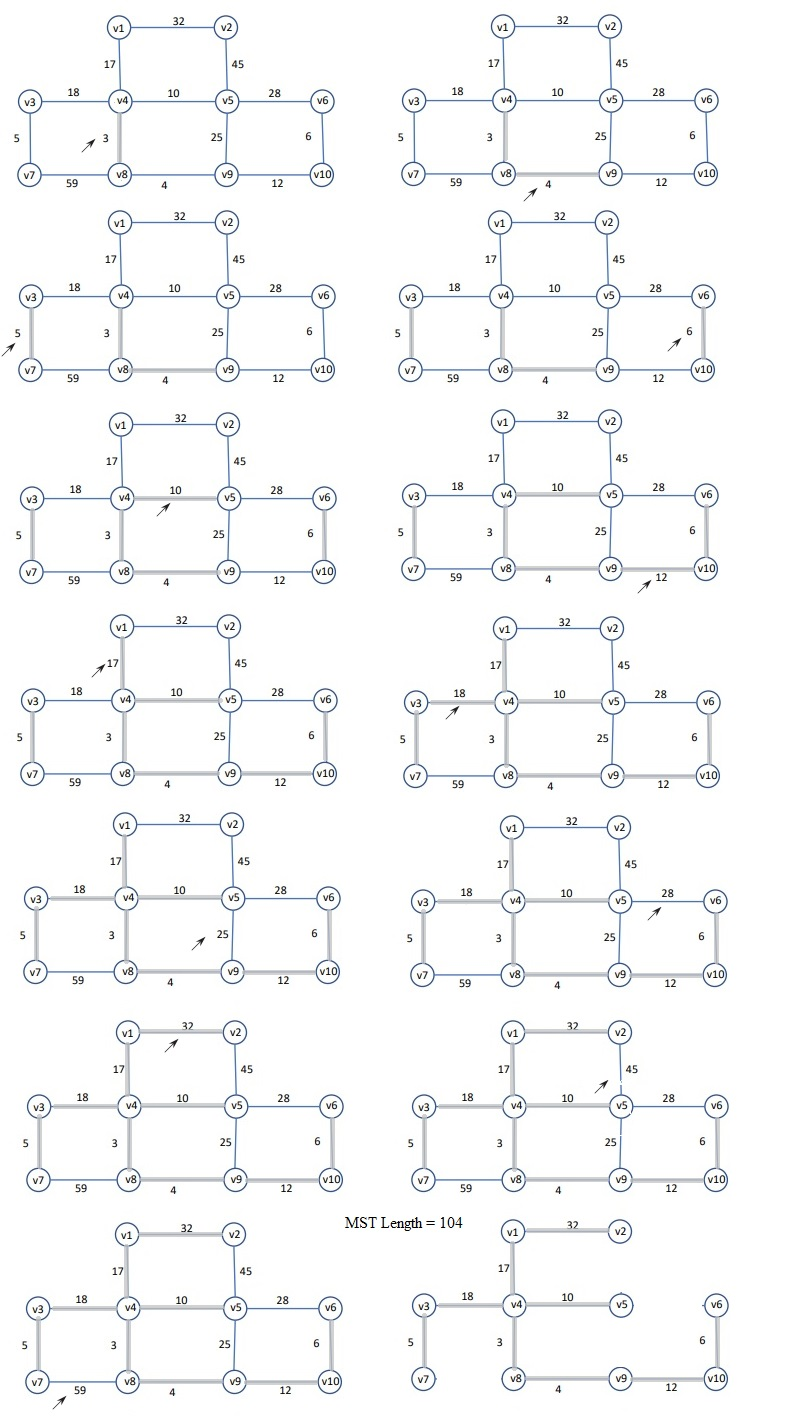
\includegraphics[width=0.6\textwidth]{kruskals.jpg}
		\end{solutionorbox}
		
		\ifprintanswers
		\newpage
		\else
		\bigskip
		\fi
		
		
		
		
		%%%%%%%%%%%%%%%%%%%%%%%%%%%%%%%%%%%%%%%%%%%%%%%%%%%%%%%%%%%%%%%%%%
		%
		% Question 
		%
		%%%%%%%%%%%%%%%%%%%%%%%%%%%%%%%%%%%%%%%%%%%%%%%%%%%%%%%%%%%%%%%%%%
		\question[5]
		Exercise 15.1-3: Consider a modification of the rod-cutting problem in which, in addition to a price $p_i$ for each rod, each cut incurs a fixed cost of $c$.  The revenue associated with a solution is now the sum of the prices of the pieces minus the costs of making the cuts.  Give a dynamic-programming algorithm to solve this modified problem.
		\begin{solutionorbox} \\ 
			Since each cut incurs a fixed cost of $c$ the new recursive solution from the textbook can be written as: \\
			$r\textsubscript{n} = \hspace{1mm}$max$(p\textsubscript{n} , r\textsubscript{1} + r\textsubscript{n-1} - c, r\textsubscript{2} + r\textsubscript{n-2} - c, ..., r\textsubscript{n-1} + r\textsubscript{1} - c)$ \\ \\ 
			Note that the profit when no cuts are made is the same. The $\proc{Bottom-Up-Cut-Rod}$ algorithm from the textbook only needs a few modifications to include the cost for cutting the rod.
			\begin{enumerate}
				\item The cost of the cut must be included as a parameter 
				\item q should be initialized to the price without cutting, not negative infinity (line 4)
				\item The inner for loop should only run until $j - 1$ because the cost of cutting should not be subtracted when no cuts are made (line 5)
				\item The cost of cutting the rod should be subtracted from the profit calculation (line 6)
			\end{enumerate} \\ Therefore, the modified algorithm is as follows: \\
			\begin{lstlisting}[mathescape=true]
			$\proc{Modified-Bottom-Up-Cut-Rod}{(p, n, c)}$
			1   let r[0..n] be a new array
			2   r[0] = 0
			3   for j = 1 to n
			4       q = p[j]
			5       for i = 1 to j - 1
			6           q = max(q, p[i] + r[j - i] - c)
			7       r[j] = q
			8   return r[n]
			
			\end{lstlisting} \\
			
		\end{solutionorbox}
		
		\ifprintanswers
		\newpage
		\else
		\bigskip
		\fi
		
		
		%%%%%%%%%%%%%%%%%%%%%%%%%%%%%%%%%%%%%%%%%%%%%%%%%%%%%%%%%%%%%%%%%%
		%
		% Question
		%
		%%%%%%%%%%%%%%%%%%%%%%%%%%%%%%%%%%%%%%%%%%%%%%%%%%%%%%%%%%%%%%%%%%
		\question[5]
		Exercise 15.1-4:  Modify $\proc{Memoized-Cut-Rod}$ to return not only the value but the actual solution.
		\begin{solutionorbox} \\
			Analyzing the textbook solution to return a solution using $\proc{Bottom-Up-Cut-Rod}$ we see that the key component to add to the algorithm is an array $s$ to hold the optimal size $i$ of the first piece to cut off when solving a subproblem of size $j$. An important detail to note about $\proc{Extended-Bottom-Up-Cut-Rod}$ is that it does not just compute the max value, but compares the currently computed value against q. We must make the comparison at each step to isolate the point at which we should make the cut and add it to array $s$. We can then combine the given $\proc{Print-Cut-Rod-Solution}$ algorithm with $\proc{Memoized-Cut-Rod}$ to create and extended Memoized Cut Rod that prints the solution computed from the first cut in the array $s$. Side note, although the question asks to return a solution and not necessarily print the solution, the array $s$ only holds the value of the first cut and does not give the exact lengths of all pieces of the rod, although they can be easily derived. The $\proc{Print-Cut-Rod-Solution}$ gives the lengths of each piece albeit in a verbose fashion. \\
			\begin{lstlisting}[mathescape=true]
			$\proc{Memoized-Cut-Rod}{(p, n, s)}$
			1   let r[0..n] and s[0..n] be new arrays
			2   for i = 0 to n
			3      r[i] = -$\infty$
			4   (r,s) = $\proc{Memoized-Cut-Rod-Aux}{(p,n,r,s)}$
			5   while n > 0
			6      print s[n]
			7      n = n - s[n]
			\end{lstlisting}
			\\
			\begin{lstlisting}[mathescape=true]
			$\proc{Memoized-Cut-Rod-Aux}{(p,n,r,s}$
			1  if r[n] $\geq$ 0
			2      return r[n]
			3  if n == 0
			4      q = 0
			5  else q = -$\infty$
			6      for i = 1 to n
			7      (cur, s) = $\proc{Memoized-Cut-Rod-Aux}{(p,n - i, r, s))}$
			8      if q < p[i] + cur
			9          q = p[i] + cur
			10         s[n] = i
			11 r[n] = q
			12 return q and s
			\end{lstlisting}
		\end{solutionorbox}
		
		\ifprintanswers
		\newpage
		\else
		\bigskip
		\fi
		
		
		%%%%%%%%%%%%%%%%%%%%%%%%%%%%%%%%%%%%%%%%%%%%%%%%%%%%%%%%%%%%%%%%%%
		%
		% Question
		%
		%%%%%%%%%%%%%%%%%%%%%%%%%%%%%%%%%%%%%%%%%%%%%%%%%%%%%%%%%%%%%%%%%%
		\question[5]
		Exercise 15.2-1: Find an optimal parenthesization of the matrix-chain product whose sequence of dimensions is: $\langle 5, 10, 3, 12, 5, 50, 6 \rangle.$ Show your work.  Use the algorithm.
		\begin{solutionorbox} \\ 
			Given the input sequence p, we have: \\
			p\textsubscript{0} = 5, p\textsubscript{1} = 10, p\textsubscript{2} = 3, p\textsubscript{3} = 12, p\textsubscript{4} = 5, p\textsubscript{5} = 50, p\textsubscript{6} = 6 \\ \\
			\begin{tabular}{c | c c c c c c}
				matrix & A\textsubscript{1} & A\textsubscript{2} & A\textsubscript{3} & A\textsubscript{4} & A\textsubscript{5} & A\textsubscript{6}\\ 
				\hline
				dimension & $5 \times 10$ & $10 \times 3$ & $3 \times 12$ & $12 \times 5$ & $5 \times 50$ & $50 \times 6$
			\end{tabular} \\ \\
			Using equation 15.7 of the textbook we have: \\
			$m[1,1] = m[2,2] = m[3,3] = m[4,4] = m[5,5] = m[6,6] = 0$ \\
			$m[1,2] = m[1,1] + m[2,2] + p\textsubscript{0}p\textsubscript{1}p\textsubscript{2} = 0 + 0 + 5 \times 10 \times 3 = 150$\\
			$m[2,3] = m[2,2] + m[3,3] + p\textsubscript{1}p\textsubscript{2}p\textsubscript{3} = 0 + 0 + 10 \times 3 \times 12 = 360$\\
			$m[3,4] = m[3,3] + m[4,4] + p\textsubscript{2}p\textsubscript{3}p\textsubscript{4} = 0 + 0 + 3 \times 12 \times 5 = 180$\\
			$m[4,5] = m[4,4] + m[5,5] + p\textsubscript{3}p\textsubscript{4}p\textsubscript{5} = 0 + 0 + 12 \times 5 \times 50 = 3000$\\
			$m[5,6] = m[5,5] + m[6,6] + p\textsubscript{4}p\textsubscript{5}p\textsubscript{6} = 0 + 0 + 5 \times 50 \times 6 = 1500$\\
			$m[1,3] = 
			min\cases{
				k = 1 & m[1,1] + m[2,3] + p\textsubscript{0}p\textsubscript{1}p\textsubscript{3} = 0 + 360 + (5 \times 10 \times 12) = 960  \cr
				k = 2 & \bf{m[1,2] + m[3,3] + p\textsubscript{0}p\textsubscript{2}p\textsubscript{3} = 150 + 0 + (5 \times 3 \times 12) = 330}  \cr
			}$\\
			$m[2,4] = 
			min\cases{
				k = 2 & \bf{m[2,2] + m[3,4] + p\textsubscript{1}p\textsubscript{2}p\textsubscript{4} = 0 + 180 + (10 \times 3 \times 5) = 330} \cr
				k = 3 & m[2,3] + m[4,4] + p\textsubscript{1}p\textsubscript{3}p\textsubscript{4} = 360 + 0 + (10 \times 12 \times 5) = 960 \cr 
			}$\\
			$m[3,5] = 
			min\cases{
				k = 3 & m[3,3] + m[4,5] + p\textsubscript{2}p\textsubscript{3}p\textsubscript{5} = 0 + 3000 + (3 \times 12 \times 50) = 4800 \cr
				k = 4 & \bf{m[3,4] + m[5,5] + p\textsubscript{2}p\textsubscript{4}p\textsubscript{5} = 180 + 0 + (3 \times 5 \times 50) = 930} \cr 
			}$\\
			$m[4,6] = 
			min\cases{
				k = 4 & \bf{m[4,4] + m[5,6] + p\textsubscript{3}p\textsubscript{4}p\textsubscript{6} = 0 + 1500 + (12 \times 5 \times 6) = 1860} \cr
				k = 5 & m[4,5] + m[6,6] + p\textsubscript{3}p\textsubscript{5}p\textsubscript{6} = 3000 + 0 + (12 \times 50 \times 6) = 6600 \cr 
			}$\\
			$m[1,4] = 
			min\cases{
				k = 1 & m[1,1] + m[2,4] + p\textsubscript{0}p\textsubscript{1}p\textsubscript{4} = 0 + 330 + (5 \times 10 \times 5) = 580  \cr
				k = 2 & \bf{m[1,2] + m[3,4] + p\textsubscript{0}p\textsubscript{2}p\textsubscript{4} = 150 + 180 + (5 \times 3 \times 5) = 405}  \cr
				k = 3 & m[1,3] + m[4,4] + p\textsubscript{0}p\textsubscript{3}p\textsubscript{4} = 330 + 0 + (5 \times 12 \times 5) = 630 \cr
			}$\\
			$m[2,5] = 
			min\cases{
				k = 2 & \bf{m[2,2] + m[3,5] + p\textsubscript{1}p\textsubscript{2}p\textsubscript{5} = 0 + 930 + (10 \times 3 \times 50) = 2430}  \cr
				k = 3 & m[2,3] + m[4,5] + p\textsubscript{1}p\textsubscript{3}p\textsubscript{5} = 360 + 180 + (10 \times 12 \times 50) = 9360  \cr
				k = 4 & m[2,4] + m[5,5] + p\textsubscript{1}p\textsubscript{4}p\textsubscript{5} = 330 + 0 + (10 \times 5 \times 50) = 2830 \cr
			}$\\
			$m[3,6] = 
			min\cases{
				k = 3 & m[3,3] + m[4,6] + p\textsubscript{2}p\textsubscript{3}p\textsubscript{6} = 0 + 1860 + (3 \times 12 \times 6) = 2076  \cr
				k = 4 & \bf{m[3,4] + m[5,6] + p\textsubscript{2}p\textsubscript{4}p\textsubscript{6} = 180 + 1500 + (3 \times 5 \times 6) = 1770}  \cr
				k = 5 & m[3,5] + m[6,6] + p\textsubscript{2}p\textsubscript{5}p\textsubscript{6} = 930 + 0 + (3 \times 50 \times 6) = 1830 \cr
			}$\\
			$m[1,5] = 
			min\cases{
				k = 1 & m[1,1] + m[2,5] + p\textsubscript{0}p\textsubscript{1}p\textsubscript{5} = 0 + 2430 + (5 \times 10 \times 50) = 4930  \cr
				k = 2 & m[1,2] + m[3,5] + p\textsubscript{0}p\textsubscript{2}p\textsubscript{5} = 150 + 930 + (5 \times 3 \times 50) = 1830  \cr
				k = 3 & m[1,3] + m[4,5] + p\textsubscript{0}p\textsubscript{3}p\textsubscript{5} = 330 + 3000 + (5 \times 12 \times 50) = 6330 \cr
				k = 4 & \bf{m[1,4] + m[5,5] + p\textsubscript{0}p\textsubscript{4}p\textsubscript{5} = 405 + 0 + (5 \times 5 \times 50) = 1655} \cr
			}$\\
			$m[2,6] = 
			min\cases{
				k = 2 & \bf{m[2,2] + m[3,6] + p\textsubscript{1}p\textsubscript{2}p\textsubscript{6} = 0 + 1770 + (10 \times 3 \times 6) = 1950}  \cr
				k = 3 & m[2,3] + m[4,6] + p\textsubscript{1}p\textsubscript{3}p\textsubscript{6} = 360 + 1860 + (10 \times 12 \times 6) = 2940  \cr
				k = 4 & m[2,4] + m[5,6] + p\textsubscript{1}p\textsubscript{4}p\textsubscript{6} = 330 + 1500 + (10 \times 5 \times 6) = 2130 \cr
				k = 5 & m[2,5] + m[6,6] + p\textsubscript{1}p\textsubscript{5}p\textsubscript{6} = 2430 + 0 + (10 \times 50 \times 6) = 5430 \cr
			}$\\
			$m[1,6] = 
			min\cases{
				k = 1 & m[1,1] + m[2,6] + p\textsubscript{0}p\textsubscript{1}p\textsubscript{6} = 0 + 1950 + (5 \times 10 \times 6) = 2250  \cr
				k = 2 & \bf{m[1,2] + m[3,6] + p\textsubscript{0}p\textsubscript{2}p\textsubscript{6} = 150 + 1770 + (5 \times 3 \times 6) = 2010}  \cr
				k = 3 & m[1,3] + m[4,6] + p\textsubscript{0}p\textsubscript{3}p\textsubscript{6} = 330 + 1860 + (5 \times 12 \times 6) = 2550 \cr
				k = 4 & m[1,4] + m[5,6] + p\textsubscript{0}p\textsubscript{4}p\textsubscript{6} = 405 + 1500 + (5 \times 5 \times 6) = 2055 \cr
				k = 5 & m[1,5] + m[6,6] + p\textsubscript{0}p\textsubscript{5}p\textsubscript{6} = 1655 + 0 + (5 \times 50 \times 6) = 3155 \cr
			}$\\ \\
			We can now construct the m and s tables using the above calculations: \\
			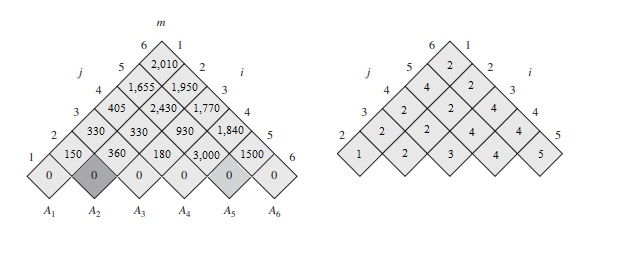
\includegraphics[width=1\textwidth]{matrixmult.jpg} \\
			Using the $\proc{Print-Optimal-Parens}{(s,1,6)}$ routine (using the help of a python program) we can now find the optimal solution:\\
			i = 1, j = 6 $\longrightarrow$ print "(" \\
			i = 1, j = 2 $\longrightarrow$ print "(" \\
			i = 1, j = 1 $\longrightarrow$ print  "A\textsubscript{1}"\\
			i = 2, j = 2 $\longrightarrow$ print "A\textsubscript{2}" \\
			Reached  print ")" \\
			i = 3, j = 6 $\longrightarrow$ print "(" \\
			i = 3, j = 4 $\longrightarrow$ print "(" \\
			i = 3, j = 3 $\longrightarrow$ print "A\textsubscript{3}" \\
			i = 4, j = 4 $\longrightarrow$ print "A\textsubscript{4}" \\
			Reached print ")" \\
			i = 5, j = 6 $\longrightarrow$ print "(" \\
			i = 5, j = 5 $\longrightarrow$ print "A\textsubscript{5}"\\
			i = 6, j = 6 $\longrightarrow$ print "A\textsubscript{6}"\\
			Reached print ")" \\
			Reached print ")" \\
			Reached print ")" \\
			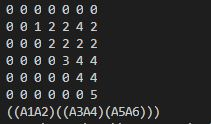
\includegraphics[width=0.5\textwidth]{parens.JPG}\\
			This shows that the optimal parenthesizing of the matrices is: \\ ((A\textsubscript{1}A\textsubscript{2})((A\textsubscript{3}A\textsubscript{4})(A\textsubscript{5}A\textsubscript{6})))\\ With a minimum total of 2,010 multiplications.
		\end{solutionorbox}
		
		\ifprintanswers
		\newpage
		\else
		\bigskip
		\fi
		
		%%%%%%%%%%%%%%%%%%%%%%%%%%%%%%%%%%%%%%%%%%%%%%%%%%%%%%%%%%%%%%%%%%
		%
		% Question 
		%
		%%%%%%%%%%%%%%%%%%%%%%%%%%%%%%%%%%%%%%%%%%%%%%%%%%%%%%%%%%%%%%%%%%
		\question[5]
		Determine the LCS of $\langle 1, 0, 0, 1, 0, 1, 0, 1 \rangle$ and $\langle 0, 1, 0, 1, 1, 0, 1, 1, 0 \rangle$
		\begin{solutionorbox} \\
			Using the $\proc{LCS-Length}{(X,Y)}$ routine with $X = 8$ and $Y = 9$ gives us the following table: \\
			\begin{tabular}{c c | c | c | c | c | c | c | c | c | c | c |}
				\multicolumn{1}{c}{\null} & \multicolumn{1}{c}{j} &
				\multicolumn{1}{c}{0} &
				\multicolumn{1}{c}{1} &
				\multicolumn{1}{c}{2} &
				\multicolumn{1}{c}{3} &
				\multicolumn{1}{c}{4} &
				\multicolumn{1}{c}{5} &
				\multicolumn{1}{c}{6} &
				\multicolumn{1}{c}{7} &
				\multicolumn{1}{c}{8} &
				\multicolumn{1}{c}{9}\\
				\multirow{1}{*}{i} & 
				\multicolumn{1}{c}{\null} &
				\multicolumn{1}{c}{y\textsubscript{j}} &
				\multicolumn{1}{c}{0} &
				\multicolumn{1}{c}{1} &
				\multicolumn{1}{c}{0} &
				\multicolumn{1}{c}{1} &
				\multicolumn{1}{c}{1} &
				\multicolumn{1}{c}{0} &
				\multicolumn{1}{c}{1} &
				\multicolumn{1}{c}{1} &
				\multicolumn{1}{c}{0}\\    
				\cline{3-12}
				\multirow{1}{*}{0} &
				x\textsubscript{i} & 0 & 0 & 0 & 0 & 0 & 0 & 0 & 0 & 0 & 0\\\cline{3-12}
				\multirow{1}{*}{1} &
				1 & 0 & 0 $\uparrow$ & 1 $\nwarrow$ & 1 $\leftarrow$ & 1 $\nwarrow$ & 1 $\nwarrow$ & 1 $\leftarrow$ & 1 $\nwarrow$ & 1 $\nwarrow$ & 1 $\leftarrow$\\\cline{3-12}
				\multirow{1}{*}{2} &
				0 & 0 & 1 $\nwarrow$ & 1 $\uparrow$ & 2 $\nwarrow$ & 2 $\leftarrow$ & 2 $\leftarrow$ & 2 $\nwarrow$ & 2 $\leftarrow$ & 2 $\leftarrow$ & 2 $\nwarrow$\\\cline{3-12}
				\multirow{1}{*}{3} &
				0 & 0 & 1 $\nwarrow$ & 1 $\uparrow$ & 2 $\nwarrow$ & 2 $\uparrow$ & 2 $\uparrow$ & 3 $\nwarrow$ & 3 $\leftarrow$ & 3 $\leftarrow$ & 3 $\nwarrow$\\\cline{3-12}
				\multirow{1}{*}{4} &
				1 & 0 & 1 $\uparrow$ & 2 $\nwarrow$ & 2 $\uparrow$ & 3 $\nwarrow$ & 3 $\nwarrow$ & 3 $\uparrow$ & 4 $\nwarrow$ & 4 $\nwarrow$ & 4 $\leftarrow$\\\cline{3-12}
				\multirow{1}{*}{5} &
				0 & 0 & 1 $\nwarrow$ & 2 $\uparrow$ & 3 $\nwarrow$ & 3 $\uparrow$ & 3 $\uparrow$ & 4 $\nwarrow$ & 4 $\uparrow$ & 4 $\uparrow$ & 5 $\nwarrow$\\\cline{3-12}
				\multirow{1}{*}{6} &
				1 & 0 & 1 $\uparrow$ & 2 $\nwarrow$ & 3 $\uparrow$ & 4 $\nwarrow$ & 4 $\nwarrow$ & 4 $\uparrow$ & 5 $\nwarrow$ & 5 $\nwarrow$ & 5 $\uparrow$\\\cline{3-12}
				\multirow{1}{*}{7} &
				0 & 0 & 1 $\nwarrow$ & 2 $\uparrow$ & 3 $\nwarrow$ & 4 $\uparrow$ & 4 $\uparrow$ & 5 $\nwarrow$ & 5 $\uparrow$ & 5 $\uparrow$ & 6 $\nwarrow$\\\cline{3-12}
				\multirow{1}{*}{8} &
				1 & 0 & 1 $\uparrow$ & 2 $\nwarrow$ & 3 $\uparrow$ & 4 $\nwarrow$ & 5 $\nwarrow$ & 5 $\uparrow$ & 6 $\nwarrow$ & 6 $\nwarrow$ & 6 $\uparrow$ \\\cline{3-12}\
			\end{tabular} \\
			Using the derived table to find the correct path, appending cells containing "$\nwarrow$" to the final set, starting at (8,9) gives the following LCS: \\
			(7,9) = 0 \\
			(6,8) = 1 \\
			(4,7) = 1 \\
			(3,6) = 0 \\
			(2,3) = 0 \\
			(1,2) = 1 \\ \\
			LCS = $\langle 1,0,0,1,1,0 \rangle$
			
			
		\end{solutionorbox}
		
		\ifprintanswers
		\newpage
		\else
		\bigskip
		\fi
		
		
		%%%%%%%%%%%%%%%%%%%%%%%%%%%%%%%%%%%%%%%%%%%%%%%%%%%%%%%%%%%%%%%%%%
		%
		% Question
		%
		%%%%%%%%%%%%%%%%%%%%%%%%%%%%%%%%%%%%%%%%%%%%%%%%%%%%%%%%%%%%%%%%%%
		\question (Extra Credit 7 points added to your exam 1 grade)
		Use Huffman's algorithm to construct an optimal binary prefix code for the letters in the following table.
		
		\begin{tabular}{|c|c|c|c|c|c|c|c|}
			\hline
			Letter    & c    & e    & i    & r    & s    & t    & x    \\ \hline
			Frequency & 0.11 & 0.22 & 0.16 & 0.12 & 0.15 & 0.10 & 0.14 \\ \hline
		\end{tabular}
		
		Encode each word using your binary code.
		\begin{enumerate}
			\item rice
			\item exit
			\item texts
			\item exercises
		\end{enumerate}
		
		\begin{solutionorbox} \\
			Using Huffman's algorithm and showing the table construction based on figure 16.5 gives the following optimal prefix codes (figure shown on next page): \\
			t = 000 \\
			c = 001 \\
			r = 100 \\
			x = 101 \\
			s = 110 \\
			i = 111 \\
			e = 01 \\
			So the following words can be encoded as follows:
			\begin{enumerate}
				\item rice = 100 111 001 01 = 10011100101
				\item exit = 01 101 111 000 = 01101111000 
				\item texts = 000 01 101 000 110 = 00001101000110
				\item exercises = 01 101 01 100 001 111 110 01 110 = 011010110000111111001110
			\end{enumerate}
			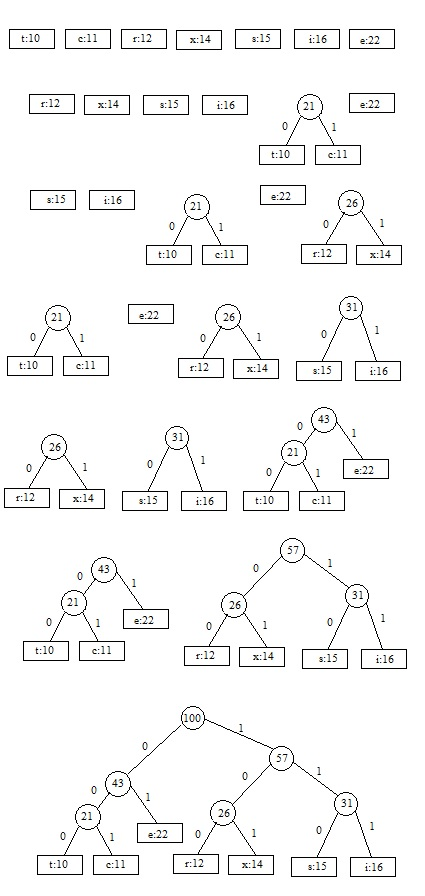
\includegraphics[width=0.6\textwidth]{huffmans.jpg}
		\end{solutionorbox}
		
		\ifprintanswers
		\newpage
		\else
		\bigskip
		\fi
		
		%%%%%%%%%%%%%%%%%%%%%%%%%%%%%%%%%%%%%%%%%%%%%%%%%%%%%%%%%%%%%%%%%%
		%
		% Question
		%
		%%%%%%%%%%%%%%%%%%%%%%%%%%%%%%%%%%%%%%%%%%%%%%%%%%%%%%%%%%%%%%%%%%
		\question (Extra credit 8 points added to your exam 1 grade)
		Implement Huffman's algorithm using Python and run it on problem.
		\begin{solutionorbox} \\
			\begin{verbatim}
			import heapq
			
			class heapnode:
			def __init__(self, char, freq):
			self.char = char
			self.freq = freq
			self.left = None
			self.right = None
			def __lt__(self, other):
			return self.freq < other.freq
			
			codes = {}
			
			def make_heap():
			print("Enter character:frequency(out of 100) separated by commas")
			print("Example: t:10, c:11, r:12, x:14, s:15, i:16, e:22")
			s2e = input()
			s2e = s2e.replace(':', ',')
			s2e = s2e.replace(' ', '')
			s2e = s2e.split(',')
			pq = []
			for i in range(0, len(s2e), 2):
			node = heapnode(s2e[i], int(s2e[i+1]))
			heapq.heappush(pq, node)
			return pq  
			
			def create_tree(pq):
			n = len(pq)
			while len(pq) > 1:
			left = heapq.heappop(pq)
			right = heapq.heappop(pq)
			merge = heapnode(None, left.freq + right.freq)
			merge.left = left
			merge.right = right
			heapq.heappush(pq, merge)
			return(heapq.heappop(pq))
			
			def make_codes(root):
			cur_code = ""
			make_codes_aux(root, cur_code)
			
			def make_codes_aux(root, cur_code):
			if (root == None):
			return
			if (root.char != None):
			codes[root.char] = cur_code
			return
			make_codes_aux(root.left, cur_code + "0")
			make_codes_aux(root.right, cur_code + "1")
			
			def accept_words():
			print("Enter words to encode only containing encoded letters 
			('quit' to terminate)")
			while 1:
			word = input()
			if (word == 'quit'):
			return
			else:
			encode_words(word)
			
			def encode_words(word):
			encoded_word = ""
			for character in word:
			encoded_word += codes[character]
			print(encoded_word)
			
			def __main__():
			heap = make_heap()
			root = create_tree(heap) 
			make_codes(root) 
			print(codes)
			accept_words()
			
			__main__()
			\end{verbatim} \\
			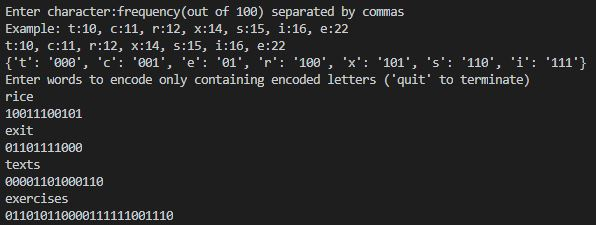
\includegraphics[width=1\textwidth]{huffmanpython.JPG}
		\end{solutionorbox}
		
		
		
		
	\end{questions}
\end{document}
